%%%%%%%%%%%%%%%%%%%%%%%%%%%%%%%%%%%%%%%%%%%%%%%%%%%%%%%%%%%%%%%%%%%%%
% LaTeX Template: Project Titlepage Modified (v 0.1) by rcx
%
% Original Source: http://www.howtotex.com
% Date: February 2014
% 
% This is a title page template which be used for articles & reports.
% 
% This is the modified version of the original Latex template from
% aforementioned website.
% 
%%%%%%%%%%%%%%%%%%%%%%%%%%%%%%%%%%%%%%%%%%%%%%%%%%%%%%%%%%%%%%%%%%%%%%

\documentclass[12pt]{report}
\usepackage[a4paper]{geometry}
\usepackage[myheadings]{fullpage}
\usepackage{fancyhdr}
\usepackage{lastpage}
\usepackage{graphicx, wrapfig, subcaption, setspace, booktabs}
\usepackage[T1]{fontenc}
\usepackage[font=small, labelfont=bf]{caption}
\usepackage{fourier}
\usepackage[protrusion=true, expansion=true]{microtype}
\usepackage[english]{babel}
\usepackage{sectsty}
\usepackage{url, lipsum}
\usepackage{tgbonum}
\usepackage{hyperref}
\usepackage{xcolor}
\usepackage{booktabs}
\usepackage{pgfplots}
\usepackage{tcolorbox}

\newcommand{\HRule}[1]{\rule{\linewidth}{#1}}
\onehalfspacing
\setcounter{tocdepth}{5}
\setcounter{secnumdepth}{5}
\pgfplotsset{width=7cm,compat=1.8}

%-------------------------------------------------------------------------------
% HEADER & FOOTER
%-------------------------------------------------------------------------------
\pagestyle{fancy}
\fancyhf{}
\setlength\headheight{15pt}
\fancyhead[R]{Open Source FPGA toolchains}
\fancyfoot[R]{Page \thepage\ of \pageref{LastPage}}
%-------------------------------------------------------------------------------
% TITLE PAGE
%-------------------------------------------------------------------------------

\begin{document}
{\fontfamily{serif}\selectfont
\title{  \textsc{Open Source FPGA toolchains}
		\\ [2.0cm]
		\HRule{0.5pt} \\
		\LARGE \textbf{\uppercase{Final Report}
		\HRule{2pt} \\ [0.5cm]
		\normalsize May 11, 2019 \vspace*{5\baselineskip}}
		}

\date{}

\author{
		Ilias Daradimos \\ 
		}

\maketitle
\tableofcontents
\newpage

%-------------------------------------------------------------------------------
% Section title formatting
\sectionfont{\scshape}
%-------------------------------------------------------------------------------

%-------------------------------------------------------------------------------
% BODY
%-------------------------------------------------------------------------------

\chapter{Scope}
The main scope of this activity is to act as a foundation for FPGA related sub-activities by testing available open source tool chains for FPGA programming with a selection of popular FPGA platforms.

Each tool chain will be evaluated against supported FPGA platforms in order to determine its capabilities. Focus is given on open source tool-chains while for platforms not yet supported by open source project, free or free license alternatives are explored.

During this process a basic set of FPGA programming tasks will be performed and evaluated. Simple tasks are used to evaluate tool chains on their simplest usage allowing the creation of common tasks across all the tool-chains. This will help evaluation by having a common reference design.

\chapter{Platforms Tested}
For the purpose of this evaluation, the platforms selected should have at least 7K LUTs and having active or under development open-source tool-chains or, as a last resort,  free toolchains.
\begin{enumerate}
    \item {Lattice ICE40}
    \newline Devboard: TinyFPGA BX
    \newline FPGA: ICE40LP8K
    \item Lattice ECP5
    \newline Devboard: ECP5 Evaluation Board
    \newline FPGA: LFE5UM5G-85F-8BG381
    \item Xilinx Artix-7
    \newline Devboard: Digilent Arty A7-100T Development Board
    \newline FPGA: XC7A100T-1CSG324C
    \item Intel Cyclone-V
    \newline Devboard: DE0-CV
    \newline FPGA: Cyclone V 5CEBA4F23C7N 

\end{enumerate}

\chapter{Tool-chains}

\subsection{IceStorm (iCE40)}
IceStorm is used for iCE40 bitstream creation. It relies on \textbf{yosys} for synthesis and \textbf{NextPNR} for place and route.

Supports all package variants of LP1K, LP4K, LP8K and HX1K, HX4K, HX8K, LP384 and UltraPlus devices.

Does not support iCE40 LM, Ultra and UltraLite
\subsection{Trellis (ECP5)}
Project Trellis enables a fully open-source flow for ECP5 FPGAs using \textbf{Yosys} for Verilog synthesis and \textbf{nextpnr} for place and route. Project Trellis itself provides the device database and tools for bitstream creation.

The following features are currently working in the Yosys -> nextpnr -> Trellis flow.

\begin{itemize}
\item Logic slice functionality, including carries
\item Distributed RAM inside logic slices
\item All internal interconnect
\item Basic IO, including tristate, using TRELLIS\_IO primitives. LPF files and DDR inputs/outputs
\item Block RAM, using either inference in Yosys or manual instantiation of the DP16KD primitive
\item Multipliers using manual instantiation of the MULT18X18D primitive. 
\newline Inference and more advanced DSP features are not yet supported.
\item Global networks (automatically promoted and routed in nextpnr)
\item PLLs
\item Transcievers (DCUs)
\end{itemize}

\subsection{NextPNR} 
    
NextPNR is a portable FPGA place and route tool that aims to be a vendor neutral, timing driven, FOSS FPGA place and route tool.

Currently NextPNR supports:
\begin{itemize}
\item Lattice iCE40 devices through project IceStorm
\item Lattice ECP5 devices through project Trellis, currently experimental
\item "generic" back-end for user-defined architectures, currently experimental
\item Xilinx 7 Series could be supported in the future through project X-Ray 
\end{itemize}

\subsection{X-Ray (Xilinx 7)}
Project X-Ray documents the Xilinx 7-Series FPGA architecture to enable development of open-source tools.



\subsection{Symbiflow}
Symbiflow aims to be an open source flow for generating bitstreams from Verilog. 

Since it uses Yosis, icestorm, trellis, xray and nextpnr for each of the supported platforms, device support at the same level as the underlying projects.


\subsection{IceStudio}
IceStudio is a visual editor for open FPGA boards. Built on top of the Icestorm project using Apio.

It implements Graphic design -> Verilog, PCF -> Bistream -> FPGA

It supports the following devices:

\begin{itemize}
\item HX1K
\item HX8K
\item LP8K
\item UP5K
\end{itemize}

It is the easiest to setup as it handles all the toolchain and device drivers downloads and it comes as an AppImage.

\subsection{Intel Quartus Prime Lite Edition and ModelSim - Intel FPGA Starter Edition}
This is the official software from Intel. The Lite edition comes with a free license and there is a Linux version.

\subsection{Vivaldo}
This is the official software from Xilinx. The HL WEBPack edition does not require a license and there is a Linux version.
\subsection{CubicBoard}
Cubicboard claims to be an open-source FPGA project for the Cyclone-V family.

They do provide Open Hardware under Apache 2.0 license although source files are for Protel/Altium EDA.

The provided software is a VirtualBox image of Ubuntu having Intel Quartus preinstalled.

\chapter{Programming tasks}
A set of programming tasks was planned in order to evaluate each platform. Tasks vary from simple tasks like LED blinking and counters to more advanced tasks like LVDS transceivers.

For each tasks the design complexity as well as the total time from source to bitstream were recorded. Details regarding tool-chain performance can be found in chapter \nameref{performance}

Verilog is used as a programming language although block design was preferred on tool-chains providing a block design editor.

A git repository was created in GitLab hosting all the code used in this activity. The repository is organised in per tool-chain folders with each folder containing implemented tasks.
\section{Simple programming tasks}
Simple tasks are used for having a similar design across all platforms. This helps to investigate the complexity required by each tool-chain to achieve the same task. For that reason a simple LED blinking task and a counter task was implemented. Small variations where introduced due to differences in the available development boards.

Project repository\cite{fpga-toolbox-eval-repo} is organised in per toolchain folders each containing implementation of the same task.

Under each tool-chain folder there is a LED\_Blink and SimpleCounter projects, these are the basic reference project for each evaluation. An additional GeekCounter project is included for devboards having 7-segment displays. Detailed information can be found on each project readme.md file

\section{Advanced programming tasks}
Moving to a more advanced programming task, an LVDS transceiver was to be designed aiming in testing single device loop-back through LVDS as well as  inter-device communication using a single LVDS pair. Due to time restriction this task is partly implemented.

An LVDS project can be found for Quartus and Vivado in the respective LVDS-Quartus\cite{fpga-toolbox-eval-repo-lvds-quartus} and LVDS-Vivado\cite{fpga-toolbox-eval-repo=lvds-vivado} branches of the project repository 


\chapter{Evaluation}
\section{Tool-chain capabilities}
The tool-chain support matrix depicts available platform support on current open-source projects. Projects that rely on these tool-chains like APIO or icestudio are not represented as their features are already covered.
Based on the current project progress, implemented features are shown in tables \ref{basic-tiles}, \ref{advanced-tiles} and \ref{routing}

\begin{table}[htp]
\centering
\begin{tabular}{|l|c|c|c|}
\hline
       & \multicolumn{1}{l|}{\textbf{IceStorm}} & \multicolumn{1}{l|}{\textbf{Trellis}} & \multicolumn{1}{l|}{\textbf{X-Ray}} \\ \hline
\textbf{Logic}     & Yes     & Yes & Yes \\ \hline
\textbf{Block RAM} & Yes & Yes & Partial \\ \hline
\end{tabular}
\caption{Basic Tiles}
\label{basic-tiles}
\end{table}


\begin{table}[htp]
\centering
\begin{tabular}{|l|c|c|c|}
\hline
                     & \multicolumn{1}{l|}{\textbf{IceStorm}} & \multicolumn{1}{l|}{\textbf{Trellis}} & \multicolumn{1}{l|}{\textbf{X-Ray}} \\ \hline
\textbf{DSP}         & Yes                                    & Yes                                   & No                                  \\ \hline
\textbf{Hard Blocks} & Yes                                    & Yes                                   & No                                  \\ \hline
\textbf{Clock Tiles} & Yes                                    & Yes                                   & No                                  \\ \hline
\textbf{I/O Tiles}   & Yes                                    & Yes                                   & Partial                             \\ \hline
\end{tabular}
\caption{Advanced Tiles}
\label{advanced-tiles}
\end{table}


\begin{table}[htp]
\centering
\begin{tabular}{|l|c|c|c|}
\hline
       & \multicolumn{1}{l|}{\textbf{IceStorm}} & \multicolumn{1}{l|}{\textbf{Trellis}} & \multicolumn{1}{l|}{\textbf{X-Ray}} \\ \hline
\textbf{Logic}     & Yes     & Yes & Yes \\ \hline
\textbf{Clock} & Yes & Yes & No \\ \hline
\end{tabular}
\caption{Routing}
\label{routing}
\end{table}

Tool-chain features for open-source and free software is shown in Table \ref{features}

\begin{table}
\begin{tabular}{|l|l|l|l|l|l|l|}
\hline
\textbf{}           & \textbf{IDE} & \textbf{\begin{tabular}[c]{@{}l@{}}Block \\ Design\end{tabular}} & \textbf{\begin{tabular}[c]{@{}l@{}}Timing\\ Analysis\end{tabular}} & \textbf{Simulation} & \textbf{\begin{tabular}[c]{@{}l@{}}Pin Mapping \\ GUI\end{tabular}} & \textbf{\begin{tabular}[c]{@{}l@{}}Floorplan \\ GUI\end{tabular}} \\ \hline
\textbf{APIO}       & Yes          & No                                                               & Yes                                                                & Yes                 & No                                                                  & No                                                                \\ \hline
\textbf{icestorm}   & No           & No                                                               & External                                                           & External            &                                                                     &                                                                   \\ \hline
\textbf{icestudio}  & Yes          & Yes                                                              & No                                                                 & No                  & No                                                                  & No                                                                \\ \hline
\textbf{prjtrellis} & No           & No                                                               &                                                                    &                     &                                                                     &                                                                   \\ \hline
\textbf{Quartus}    & Yes          & Yes                                                              & Yes                                                                & Yes                 & Yes                                                                 & Yes                                                               \\ \hline
\textbf{Vivado}     & Yes          & Yes                                                              & Yes                                                                & Yes                 & Yes                                                                 & Yes                                                               \\ \hline
\end{tabular}
\caption{Features}
\label{features}
\end{table}

\section{icestorm and prjtrellis}

These are command line tools for ICE40 and ECP5 FPGA series. Each tool is responsible for a single step in the process of taking a verilog file and ending up with a programmed device. Since this is a multistep process, it is best to be carried out by using a Makefile as demonstrated in the project repository.

There is a PLL configuration tool for each platform (icepll, ecppll) that can be used for generating PLL code. As en example an 120MHz clock derived from a 12MHz clock is demonstrated:

\begin{tcolorbox}
\begin{verbatim}
$ icepll -m -f pll.v -i 12 -o 120

F_PLLIN:    12.000 MHz (given)
F_PLLOUT:  120.000 MHz (requested)
F_PLLOUT:  120.000 MHz (achieved)

FEEDBACK: SIMPLE
F_PFD:   12.000 MHz
F_VCO:  960.000 MHz

DIVR:  0 (4'b0000)
DIVF: 79 (7'b1001111)
DIVQ:  3 (3'b011)

FILTER_RANGE: 1 (3'b001)

PLL configuration written to: pll.v

\end{verbatim}
\end{tcolorbox}
This will also generate a pll module file that can be included in the project

\begin{tcolorbox}
\begin{verbatim}
/**
 * PLL configuration
 *
 * This Verilog module was generated automatically
 * using the icepll tool from the IceStorm project.
 * Use at your own risk.
 *
 * Given input frequency:        12.000 MHz
 * Requested output frequency:  120.000 MHz
 * Achieved output frequency:   120.000 MHz
 */

module pll(
	input  clock_in,
	output clock_out,
	output locked
	);

SB_PLL40_CORE #(
		.FEEDBACK_PATH("SIMPLE"),
		.DIVR(4'b0000),		// DIVR =  0
		.DIVF(7'b1001111),	// DIVF = 79
		.DIVQ(3'b011),		// DIVQ =  3
		.FILTER_RANGE(3'b001)	// FILTER_RANGE = 1
	) uut (
		.LOCK(locked),
		.RESETB(1'b1),
		.BYPASS(1'b0),
		.REFERENCECLK(clock_in),
		.PLLOUTCORE(clock_out)
		);

endmodule

\end{verbatim}
\end{tcolorbox}

Timing analysis is available for ICE40 using the icetime tool. It will report timing estimate as well as detailed timing report.

Simulation is possible by creating a testbench file and using iverilog combined with gtk-wave for visualization



\section{APIO}
APIO is a command line tool that wraps around icestorm toolchain and attempts to simplify development process. It provides all features of icestorm toolchain as well as simulation. It handles driver installation and project initialization for supported boards.

A summary of available features is presented by command usage
\begin{tcolorbox}
\begin{verbatim}
Project commands:
  build      Synthesize the bitstream.
  clean      Clean the previous generated files.
  lint       Lint the verilog code.
  sim        Launch the verilog simulation.
  time       Bitstream timing analysis.
  upload     Upload the bitstream to the FPGA.
  verify     Verify the verilog code.

Setup commands:
  drivers    Manage FPGA boards drivers.
  init       Manage apio projects.
  install    Install packages.
  uninstall  Uninstall packages.

Utility commands:
  boards     Manage FPGA boards.
  config     Apio configuration.
  examples   Manage verilog examples.
  raw        Execute commands using Apio packages.
  system     System tools.
  upgrade    Check the latest Apio version.
\end{verbatim}
\end{tcolorbox}
One drawback is that it uses the now deprecated arachne-pnr instead of its replacement nextpnr.

An Atom editor plugin is available that integrates APIO functionality and provides the same functionality from within the editor.
\begin{figure}[h!]
\includegraphics[width=1\textwidth]{Images/APIO_Atom.png}
\caption{APIO plugin for Atom}
\end{figure}
\section{IceStudio}
Icestudio is built on top of APIO and Icestorm projects and currently supports the ICE40 FPGA family. Icestudio comes as an AppImage and handles all toolchain and "Driver" (udev rules) requirements through its GUI
It is a block design editor (Figure \ref{ref:icestudio_block}) and comes with a basic set of blocks like

\begin{itemize}
\item I/O
\item Memory
\item Multiplexers
\item Gates
\item Flip-flops
\item Prescalers/Counters
\end{itemize}

\begin{figure}[ht]
\includegraphics[width=1\textwidth]{Images/icestudio_blocks.png}
\caption{Icestudio block design}
\label{ref:icestudio_block}
\end{figure}

Custom blocks can be created by implementing the underlying functionality in Verilog (Figure \ref{ref:icestudio_custom_block}) and provide input and output ports in order to connecto to other blocks
\begin{figure}[ht]
\includegraphics[width=1\textwidth]{Images/icestudio_custom_block.png}
\caption{Icestudio custom block}
\label{ref:icestudio_custom_block}
\end{figure}

Sets of blocks can be organised in collections that are ZIP files of specific file structure. Collections can be added in Icestudio extending its functionality. Collections also include example projects that can be loaded into the block editor

A list of opensource collections can be found at 

\url{https://github.com/FPGAwars/icestudio-collections}

\url{https://fpgawars.github.io/}

For creating custom collections, a tool is available assisting in creating the basic file and folder structure: \url{https://github.com/FPGAwars/icm}

\section{Quartus}
Quartus supports VHDL and Verilog source files as well as block design. It comes with a variety of IP core re-configurable generators

Quartus Prime software features include \cite{Wikipedia_Quartus}:
\begin{itemize}
\item SOPC Builder, a tool in Quartus Prime software that eliminates manual system integration tasks by automatically generating interconnect logic and creating a testbench to verify functionality
\item Qsys, a system-integration tool that is the next generation of SOPC Builder. It uses an FPGA-optimized network-on-chip architecture that doubles the fMAX performance vs. SOPC Builder.
\item SoCEDS, a set of development tools, utility programs, run-time software, and application examples to help you develop software for SoC FPGA embedded systems.
\item DSP Builder, a tool that creates a seamless bridge between the MATLAB/Simulink tool and Quartus Prime software, so FPGA designers have the algorithm development, simulation, and verification capabilities of MATLAB/Simulink system-level design tools
\item External memory interface toolkit, which identifies calibration issues and measures the margins for each DQS signal.
\item Generation of JAM/STAPL files for JTAG in-circuit device programmers.
\end{itemize}

A comparison of available features at this time is shown in 

\section{Vivado}
Vivado HL WebPACK Edition was used for this evaluation. It is provided at no cost but with device limitations.

Features available in this edition are:
\begin{itemize}
    \item Synthesis and Place and Route
    \item Dynamic Function eXchange
    \item Simulator
    \item Device Programmer
    \item Logic Analyzer
    \item Serial I/O Analyzer
    \item Debug IP (ILA/VIO/IBERT)	\item High-Level Synthesis
    \item IP Integrator
\end{itemize}

Non free editions also include System Generator for DSP and Model Composer

\chapter{Version control}
Version control is a vital tool for complex projects requiring the collaboration of several persons.
Version control tools provide the means for creating milestones in code, develop new or experimental features as well as revert changes that introduced bugs in an organized and structured way.

When several persons need to modify the content of the same file at the same time, all changes need to be merged into the final result. Such a task, done manually, would require tremendous effort, introduce new errors and in some cases is almost impossible. 

Version control allows several persons to interact and modify the same files and provides the means for all the changes to be merged in a functional outcome.  Parts of the content are assembled automatically and any conflicts in content can be handled efficiently.

\section{iCE40}
iCE40 projects can easily use git for version control. An example .gitignore file is presented. All files generated by Makefile are ignored.

\textbf{icestorm} and \textbf{APIO} .gitignore file contents
\begin{tcolorbox}
\begin{verbatim}
*.out
*.blif
*.bin
*.asc
*.vcd
*.rpt
abc.history
.sconsign.dblite
\end{verbatim}
\end{tcolorbox}

\section{ECP5}
\textbf{prjtrellis} projects can easily use git for version control. All files generated by Makefile are ignored

An example .gitignore file is presented
\begin{tcolorbox}
\begin{verbatim}
*.bit
*.svf
*.config
*.json
\end{verbatim}
\end{tcolorbox}

\section{Vivado}
Version control methods for Vivado are explained in  \href{https://www.xilinx.com/support/documentation/application_notes/xapp1165.pdf}{application note XAPP1165} where version control for project mode, non-project mode and IP are described.

An example .gitignore is provided by xilinx and was extended for latest Vivado version. It can be found in Vivado folder in the project repo.

\section{Quartus}
For Quartus an effort was made to determine the bare minimum of files needed in order for a project to be able to regenerated. 
A .gitignore file was created keeping all files necessary for project creation and IP regeneration. It can be found under Quartus folder in the project repository.

\chapter{Performance}
\label{performance}
Performance evaluation for each tool-chain is based on time taken for all steps needed to go from source to bit-stream. Each test is run twice to also measure total time on consecutive executions. This was needed as some tool-chains generate IP cores the first time used and that contributes to overall performance time.

IceStudio is using APIO under the hood so performance should be almost identical

Performance times are shown for LED Blinker project (Figure \ref{fig:led_blinker_times}) and SimpleCounter project (Figure \ref{fig:counter_times})
\begin{figure}
    \centering
    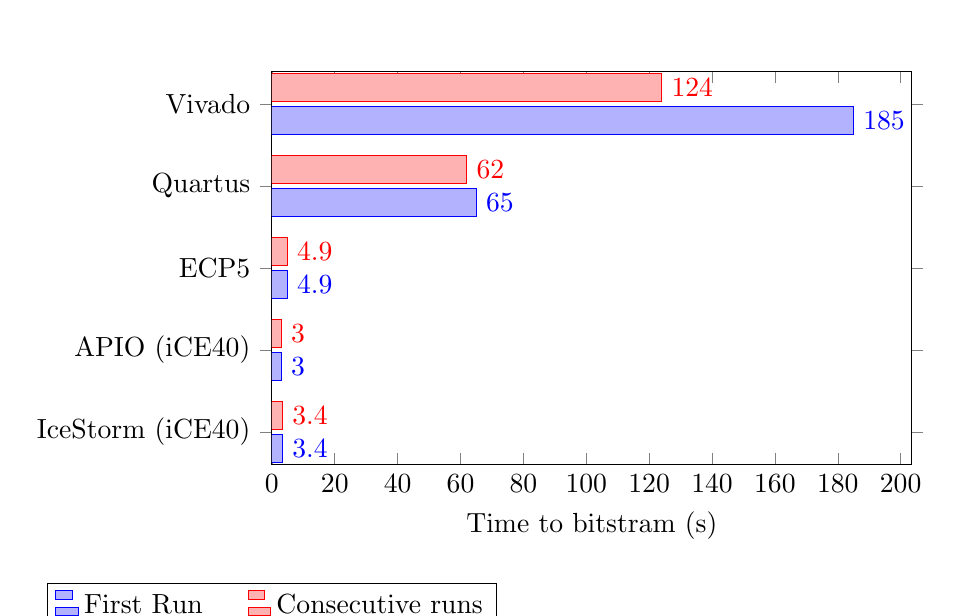
\begin{tikzpicture}
        \begin{axis}[ 
        scale only axis, % The height and width argument only apply to the actual axis
        height=5cm,
        width=\textwidth-4cm,
        xbar, xmin=0,
        xlabel={Time to bitstram (s)},
        symbolic y coords={%
            {IceStorm (iCE40)},
            {APIO (iCE40)},
            {ECP5},
            {Quartus},
            {Vivado}
            },
        ytick=data,
        nodes near coords, 
        nodes near coords align={horizontal},
        ytick=data,
        legend style={
            at={(0,-0.3)},
            anchor=north,
            legend columns=-1,
            /tikz/every even column/.append style={column sep=0.5cm}
        },
        ]
        \addplot coordinates {
            (3.4,{IceStorm (iCE40)}) 
            (3.0,{APIO (iCE40)})
            (4.9,{ECP5}) 
            (65,{Quartus}) 
            (185,{Vivado})};
        \addplot coordinates {
            (3.4,{IceStorm (iCE40)}) 
            (3.0,{APIO (iCE40)})
            (4.9,{ECP5}) 
            (62,{Quartus}) 
            (124,{Vivado})};
        \legend{First Run, Consecutive runs}
        \end{axis}
    \end{tikzpicture}
    \caption{LED Blinker time}
    \label{fig:led_blinker_times}
\end{figure}

\begin{figure}
    \centering
    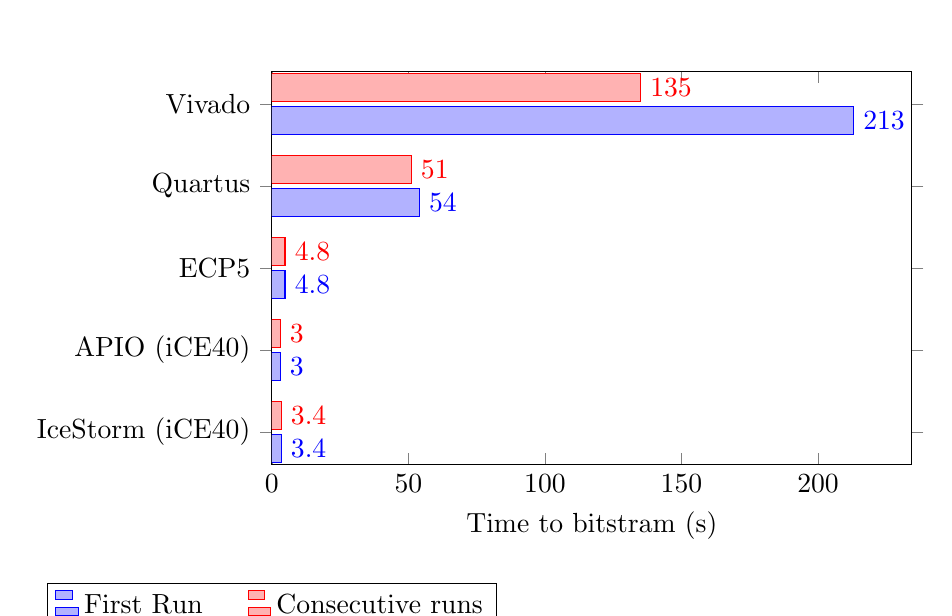
\begin{tikzpicture}
        \begin{axis}[ 
        scale only axis, % The height and width argument only apply to the actual axis
        height=5cm,
        width=\textwidth-4cm,
        xbar, xmin=0,
        xlabel={Time to bitstram (s)},
        symbolic y coords={%
            {IceStorm (iCE40)},
            {APIO (iCE40)},
            {ECP5},
            {Quartus},
            {Vivado}
            },
        ytick=data,
        nodes near coords, 
        nodes near coords align={horizontal},
        ytick=data,
        legend style={
            at={(0,-0.3)},
            anchor=north,
            legend columns=-1,
            /tikz/every even column/.append style={column sep=0.5cm}
        },
        ]
        \addplot coordinates {
            (3.4,{IceStorm (iCE40)}) 
            (3.0,{APIO (iCE40)})
            (4.8,{ECP5}) 
            (54,{Quartus}) 
            (213,{Vivado})};
        \addplot coordinates {
            (3.4,{IceStorm (iCE40)}) 
            (3.0,{APIO (iCE40)})
            (4.8,{ECP5}) 
            (51,{Quartus}) 
            (135,{Vivado})};
        \legend{First Run, Consecutive runs}
        \end{axis}
    \end{tikzpicture}
    \caption{Counter time}
    \label{fig:counter_times}
\end{figure}



\chapter{Conclusion}
\label{conclusion}
Open source ice40 and ECP5 tool-chains are mature enough for code-based development. Tools for timing and some code generation scripts are already available. Simulation visualization is possible through other open-source projects, 

APIO is a step forward towards an IDE easing development. Although it currently supports only ice40 devices the foundations for ecp5 support are well laid.

IceStudio is the only application available allowing for block design development for the ice40 family. It is still lacking many features of the commercial equivalents but being an active project one can expect that it will be on par with commercial solutions. As with APIO, an ECP5 version is likely to be possible.

Moving on to commercial solutions, Intel Quartus although initially appeared straightforward to use, there were some shortcomings. Being a project inherited from Altera, all code had to be refactored for re-branding. As it turns out this was done poorly and in some cases, users where required to alter platforms source files to overcome errors. 

User experience left mixed feelings, although steps from block design to bit-stream are very clear, block design editor needs some work as it requires some effort to keep the design clean and tidy.

Xilinx Vivado was a pleasant surprise regarding its block design editor. the interface is intuitive, blocks and connections can be managed in a way that always produces a clean and tidy design. Rearrange and align tools further help in that aspect. 
A design assistant tool is also available to further accelerate design by suggesting missing elements of a newly placed IP.

What felt a bit peculiar is the use of IPs even for simple tasks like selecting bits from a bus but it still promotes clear design UX wise.
Finally, when it comes to choosing a device family for an open-source project, options are quite clear as ice40 and ECP5 are the first candidates.

For more demanding applications an investment on Xilinx devices is suggested since an effort for Xilinx open-source tool-chains is in the works
%-------------------------------------------------------------------------------
% REFERENCES
%-------------------------------------------------------------------------------
\newpage
\bibliographystyle{IEEEtran}
\bibliography{refs}


% \begin{thebibliography}{9}
% \bibitem{Wikipedia_Quartus}
% \url{https://en.wikipedia.org/wiki/Intel_Quartus_Prime}

% \bibitem{Wikipedia_Vivado}
% \url{https://en.wikipedia.org/wiki/Xilinx_Vivado}
% \end{thebibliography}
}
\end{document}

%-------------------------------------------------------------------------------
% SNIPPETS
%-------------------------------------------------------------------------------

%\begin{figure}[!ht]
%	\centering
%	\includegraphics[width=0.8\textwidth]{file_name}
%	\caption{}
%	\centering
%	\label{label:file_name}
%\end{figure}

%\begin{figure}[!ht]
%	\centering
%	\includegraphics[width=0.8\textwidth]{graph}
%	\caption{Blood pressure ranges and associated level of hypertension (American Heart Association, 2013).}
%	\centering
%	\label{label:graph}
%\end{figure}

%\begin{wrapfigure}{r}{0.30\textwidth}
%	\vspace{-40pt}
%	\begin{center}
%		\includegraphics[width=0.29\textwidth]{file_name}
%	\end{center}
%	\vspace{-20pt}
%	\caption{}
%	\label{label:file_name}
%\end{wrapfigure}

%\begin{wrapfigure}{r}{0.45\textwidth}
%	\begin{center}
%		\includegraphics[width=0.29\textwidth]{manometer}
%	\end{center}
%	\caption{Aneroid sphygmomanometer with stethoscope (Medicalexpo, 2012).}
%	\label{label:manometer}
%\end{wrapfigure}

%\begin{table}[!ht]\footnotesize
%	\centering
%	\begin{tabular}{cccccc}
%	\toprule
%	\multicolumn{2}{c} {Pearson's correlation test} & \multicolumn{4}{c} {Independent t-test} \\
%	\midrule	
%	\multicolumn{2}{c} {Gender} & \multicolumn{2}{c} {Activity level} & \multicolumn{2}{c} {Gender} \\
%	\midrule
%	Males & Females & 1st level & 6th level & Males & Females \\
%	\midrule
%	\multicolumn{2}{c} {BMI vs. SP} & \multicolumn{2}{c} {Systolic pressure} & \multicolumn{2}{c} {Systolic Pressure} \\
%	\multicolumn{2}{c} {BMI vs. DP} & \multicolumn{2}{c} {Diastolic pressure} & \multicolumn{2}{c} {Diastolic pressure} \\
%	\multicolumn{2}{c} {BMI vs. MAP} & \multicolumn{2}{c} {MAP} & \multicolumn{2}{c} {MAP} \\
%	\multicolumn{2}{c} {W:H ratio vs. SP} & \multicolumn{2}{c} {BMI} & \multicolumn{2}{c} {BMI} \\
%	\multicolumn{2}{c} {W:H ratio vs. DP} & \multicolumn{2}{c} {W:H ratio} & \multicolumn{2}{c} {W:H ratio} \\
%	\multicolumn{2}{c} {W:H ratio vs. MAP} & \multicolumn{2}{c} {\% Body fat} & \multicolumn{2}{c} {\% Body fat} \\
%	\multicolumn{2}{c} {} & \multicolumn{2}{c} {Height} & \multicolumn{2}{c} {Height} \\
%	\multicolumn{2}{c} {} & \multicolumn{2}{c} {Weight} & \multicolumn{2}{c} {Weight} \\
%	\multicolumn{2}{c} {} & \multicolumn{2}{c} {Heart rate} & \multicolumn{2}{c} {Heart rate} \\
%	\bottomrule
%	\end{tabular}
%	\caption{Parameters that were analysed and related statistical test performed for current study. BMI - body mass index; SP - systolic pressure; DP - diastolic pressure; MAP - mean arterial pressure; W:H ratio - waist to hip ratio.}
%	\label{label:tests}
%\end{table}%\documentclass{article}
%\usepackage[utf8]{inputenc}

%\title{Weekly Report template}
%\author{gandhalijuvekar }
%\date{January 2019}

%\begin{document}

%\maketitle

%\section{Introduction}

%\end{document}
